\section{Data Used for Services and Amenities Maps}

This appendix consists of all of the Excel Spreadsheets that we created in order to map data on the services and amenities in Spartanburg. All data was hand-collected through Google Maps and data sets found through websites run by the City of Spartanburg.
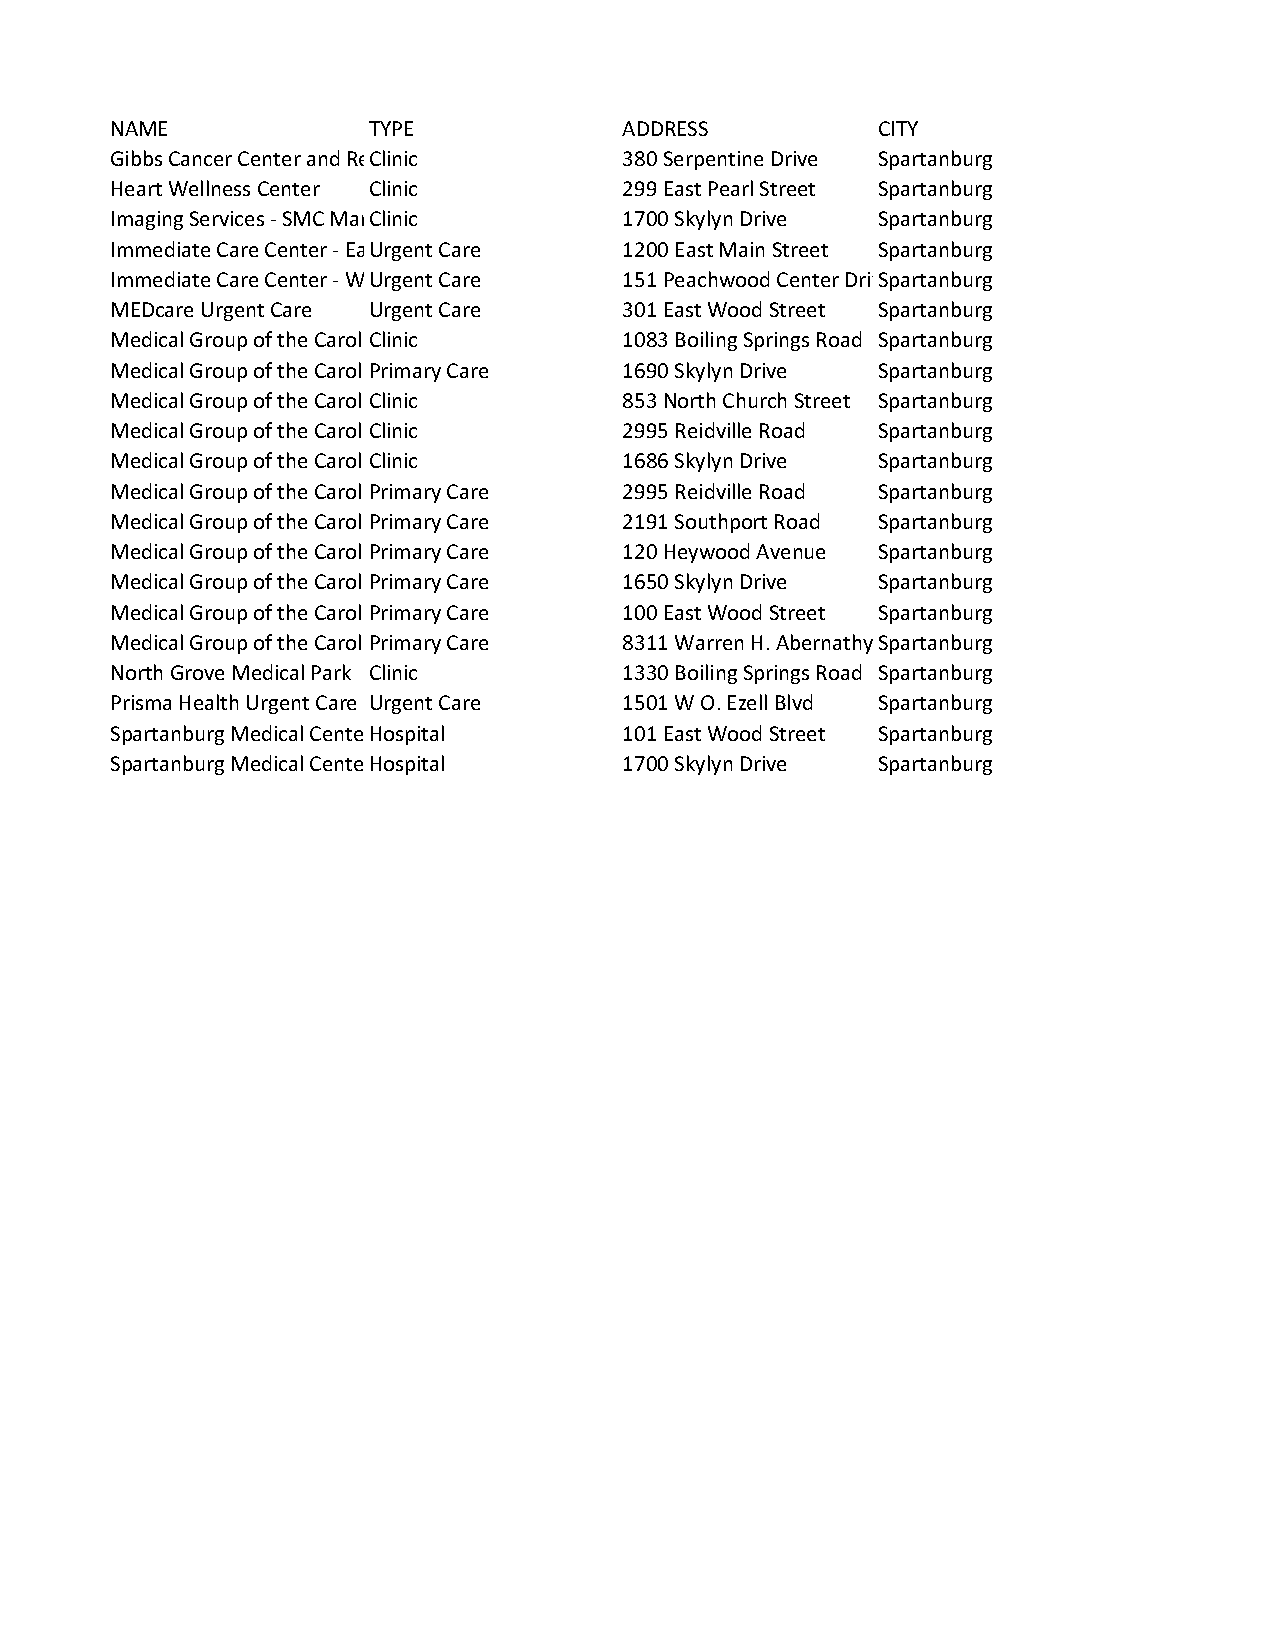
\includepdf[pages=-]{AmenitiesData.pdf}


\section{Data Collected by U.S. Census Bureau on Working Residents of Spartanburg County}

This appendix consists of the spreadsheet we obtained from the U.S. Census Bureau, which provides several summary statistics on the employed residents of Spartanburg County. In this dataset, it shows the amount of vehicles that workers reported as being available to them, as well as showing the means of transportation that workers reported using in order to get to their jobs.

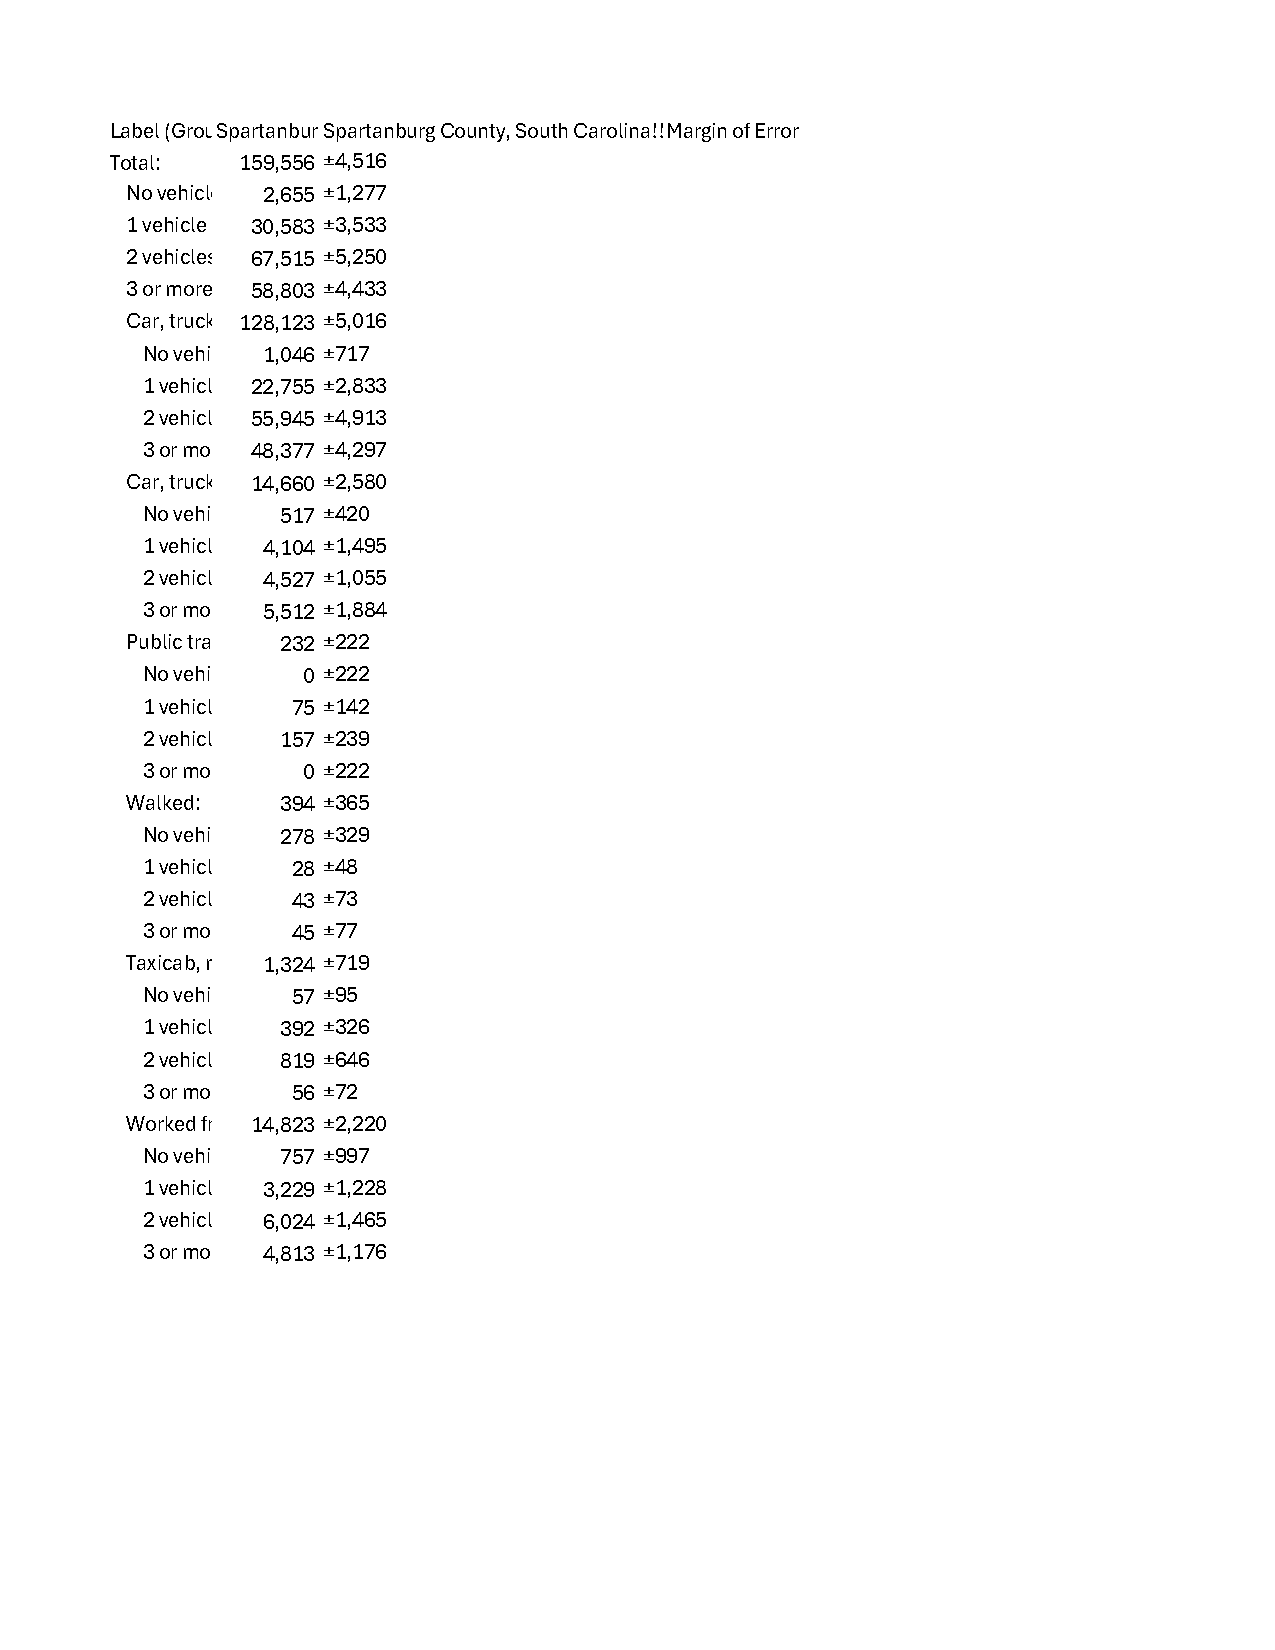
\includepdf[pages=-]{meansoftransportation.pdf}

\section{Data Summary Created for Data in Appendix B}

This appendix consists of a simple data summary that we did using Python programming tools, in order to extract and more deeply analyze the data found in Appendix B.

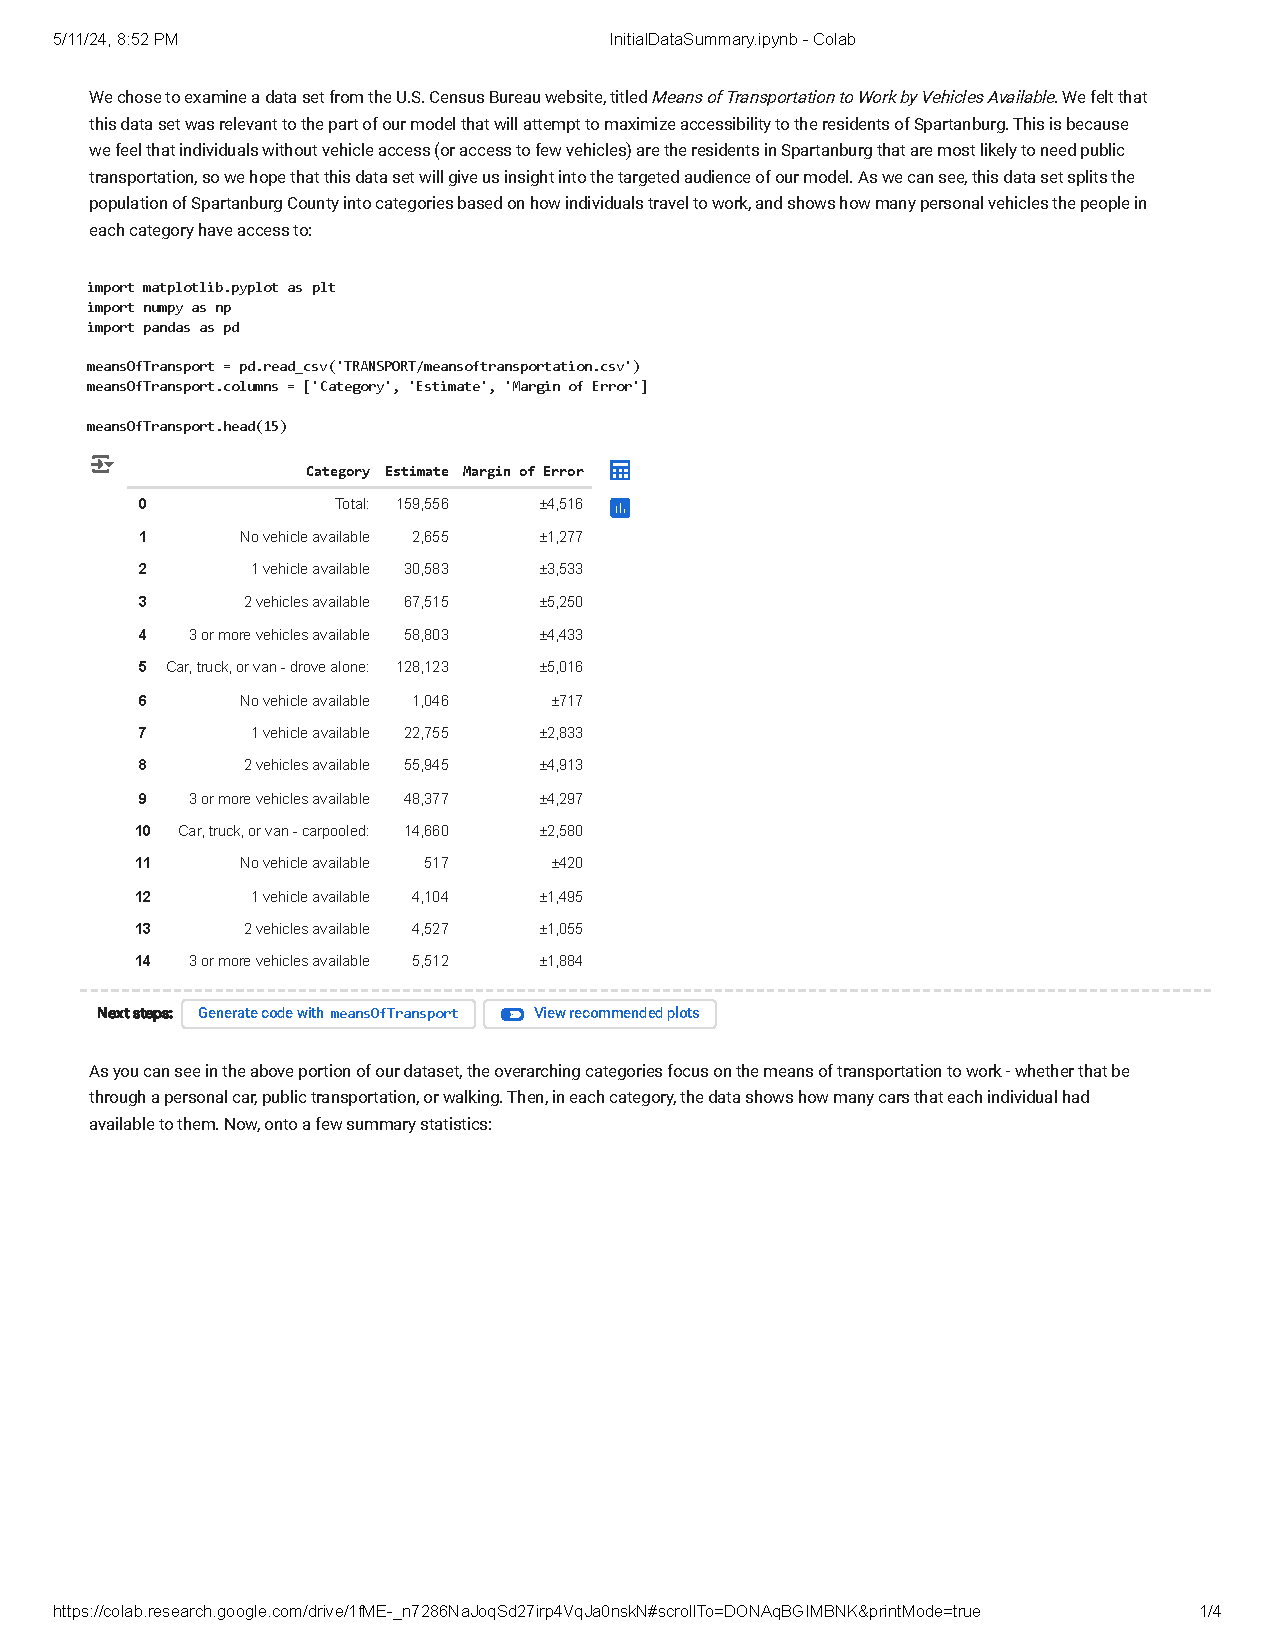
\includepdf[pages=-]{InitialDataSummary.pdf}

\section{Information on Bus Stops}

This appendix consists of a pdf file with the names of all the different bus stops, what routes they are on, and their latitude and longitude location.
\begin{figure}
    \centering
    
\includegraphics[width=1\linewidth]{GTFS stops.pdf}
\end{figure}